\documentclass[../TDAM3.tex]{subfiles}%

\begin{document}
\section{Carboglace}
\enonce{%
	À \SI{195}{K}, le dioxyde de carbone se solidifie dans une structure cristalline
	appelée \textit{carboglace}.
	\begin{tcn}(defi)<lftt>'l'{Données}
		$M_{\ce{C}} = \SI{12.0}{g.mol^{-1}}$ et $r_{\ce{C}} = \SI{77.0}{pm}$~;
		$M_{\ce{O}} = \SI{16.0}{g.mol^{-1}}$ et $r_{\ce{O}} = \SI{73.0}{pm}$.
	\end{tcn}
}%
\QR{%
	Rappeler la géométrie de la molécule de dioxyde de carbone \ce{CO2}.
}{%
	Le dioxyde de carbone a une géométrie \textbf{linéaire}.
}%

\begin{blocQR}
	\item \enonce{%
		Les atomes de carbone occupent un réseau CFC, de paramètre de maille $a
			= \SI{558}{pm}$. Les molécules s'orientent ensuite selon les diagonales des
		face du cube.
	}%
	\QR{%
		Représenter cette maille. Déterminer la population d'une maille.
	}{%
		La maille est ci-après. On a $8\times1/8+6\times1/2 = 4$ molécules
		de \ce{CO2} par maille.
		\begin{figure}[h]
			\centering
			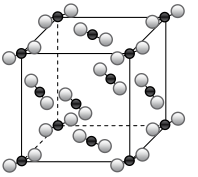
\includegraphics[scale=.8]{carboglace}
			\caption{Maille élémentaire de carboglace. Le carbone est en noir,
				l'oxygène en gris.}
			\label{fig:cbgl}
		\end{figure}
	}%

	\QR{%
		Déterminer la distance $d$ entre deux atomes de carbone voisins.
		Commenter cette valeur, par comparaison avec la longueur de la liaison
		$\ce{C=O}$ dans \ce{CO2}~: $d_{\ce{C=O}} = \SI{120}{pm}$.
	}{%
		Selon la diagonale d'une face, $2d = a \sqrt{2} \Ra \fbox{d =
				\SI{395}{pm}}$. Cette distance est la somme d'une longueur de liaison
		covalente \ce{C=O} (\SI{120}{pm}) et d'une distance entre \ce{O} d'une
		molécule et \ce{C} d'une molécule voisine~: celle-ci vaut donc
		\SI{275}{pm}, soit nettement plus que la longueur d'une liaison
		covalente. En effet, la cohésion entre molécules de \ce{CO2} est assurée
		par des forces de Van der Waals, d'énergie plus faible qu'une liaison
		covalent.
	}%
\end{blocQR}

\QR{%
	Déterminer la compacité de cette structure. On considérera que le modèle
	des sphères dures s'applique aux atomes et non à la molécule.
}{%
	La compacité est le rapport du volume occupé sur le volume de la maille.
	Ainsi, avec $N_{\ce{O}} = 8$ et $N_{\ce{C}} = 4$, on a
	\[
		C = \frac{N_{\ce{C}}\times \frac{4}{3}\pi r_{\ce{C}}^{3} +
			N_{\ce{O}}\times \frac{4}{3}\pi r_{\ce{O}}^{3} }{a^3} = \num{0.12}
	\]
}%

\QR{%
Déterminer la densité de la carboglace.
}{%
La masse volumique est
\[
	\rho = \frac{N_{\ce{C}}M_{\ce{C}} + N_{\ce{O}}M_{\ce{O}}}{\Nc_A a^3}
	= \SI{1.68e3}{kg.m ^{-3}}
\]
La densité, rapport de la masse volumique de la carboglace sur la masse
volumique de l'eau, est donc \fbox{$d = \num{1.68}$}.
}%

\end{document}
